\documentclass[journal,12pt,twocolumn]{IEEEtran}
%
\usepackage{setspace}
\usepackage{textcomp}
\usepackage{gensymb}
%\doublespacing
\singlespacing

\usepackage[cmex10]{amsmath}
\usepackage{amsthm}
%\usepackage{iithtlc}
\usepackage{mathrsfs}
\usepackage{txfonts}
\usepackage{stfloats}
\usepackage{bm}
\usepackage{cite}
\usepackage{cases}
\usepackage{subfig}
%\usepackage{xtab}
\usepackage{longtable}
\usepackage{multirow}
%\usepackage{algorithm}
%\usepackage{algpseudocode}
\usepackage{enumitem}
\usepackage{mathtools}
\usepackage{steinmetz}
\usepackage{tikz}
\usepackage{circuitikz}
\usepackage{verbatim}
\usepackage{tfrupee}
\usepackage[breaklinks=true]{hyperref}
%\usepackage{stmaryrd}
\usepackage{tkz-euclide} % loads  TikZ and tkz-base
%\usetkzobj{all}
\usetikzlibrary{calc,math}
\usepackage{listings}
    \usepackage{color}                                            %%
    \usepackage{array}                                            %%
    \usepackage{longtable}                                        %%
    \usepackage{calc}                                             %%
    \usepackage{multirow}                                         %%
    \usepackage{hhline}                                           %%
    \usepackage{ifthen}                                           %%
  %optionally (for landscape tables embedded in another document): %%
    \usepackage{lscape}     
\usepackage{multicol}
\usepackage{chngcntr}
%\usepackage{enumerate}

%\usepackage{wasysym}
%\newcounter{MYtempeqncnt}
\DeclareMathOperator*{\Res}{Res}
%\renewcommand{\baselinestretch}{2}
\renewcommand\thesection{\arabic{section}}
\renewcommand\thesubsection{\thesection.\arabic{subsection}}
\renewcommand\thesubsubsection{\thesubsection.\arabic{subsubsection}}

\renewcommand\thesectiondis{\arabic{section}}
\renewcommand\thesubsectiondis{\thesectiondis.\arabic{subsection}}
\renewcommand\thesubsubsectiondis{\thesubsectiondis.\arabic{subsubsection}}

% correct bad hyphenation here
\hyphenation{op-tical net-works semi-conduc-tor}
\def\inputGnumericTable{}                                 %%

\lstset{
%language=C,
frame=single, 
breaklines=true,
columns=fullflexible
}
\newenvironment{amatrix}[1]{%
  \left(\begin{array}{@{}*{#1}{c}|c@{}}
}{%
  \end{array}\right)
}
\DeclarePairedDelimiter\abs{\lvert}{\rvert}%
\DeclarePairedDelimiter\norm{\lVert}{\rVert}%

% Swap the definition of \abs* and \norm*, so that \abs
% and \norm resizes the size of the brackets, and the 
% starred version does not.
\makeatletter
\let\oldabs\abs
\def\abs{\@ifstar{\oldabs}{\oldabs*}}
%
\let\oldnorm\norm
\def\norm{\@ifstar{\oldnorm}{\oldnorm*}}
\makeatother

\newtheorem{theorem}{Theorem}[section]
\newtheorem{problem}{Problem}
\newtheorem{proposition}{Proposition}[section]
\newtheorem{lemma}{Lemma}[section]
\newtheorem{corollary}[theorem]{Corollary}
\newtheorem{example}{Example}[section]
\newtheorem{definition}[problem]{Definition}
%\newtheorem{thm}{Theorem}[section] 
%\newtheorem{defn}[thm]{Definition}
%\newtheorem{algorithm}{Algorithm}[section]
%\newtheorem{cor}{Corollary}
\newcommand{\BEQA}{\begin{eqnarray}}
\newcommand{\EEQA}{\end{eqnarray}}
\newcommand{\define}{\stackrel{\triangle}{=}}
\bibliographystyle{IEEEtran}
%\bibliographystyle{ieeetr}
\providecommand{\mbf}{\mathbf}
\providecommand{\pr}[1]{\ensuremath{\Pr\left(#1\right)}}
\providecommand{\qfunc}[1]{\ensuremath{Q\left(#1\right)}}
\providecommand{\sbrak}[1]{\ensuremath{{}\left[#1\right]}}
\providecommand{\lsbrak}[1]{\ensuremath{{}\left[#1\right.}}
\providecommand{\rsbrak}[1]{\ensuremath{{}\left.#1\right]}}
\providecommand{\brak}[1]{\ensuremath{\left(#1\right)}}
\providecommand{\lbrak}[1]{\ensuremath{\left(#1\right.}}
\providecommand{\rbrak}[1]{\ensuremath{\left.#1\right)}}
\providecommand{\cbrak}[1]{\ensuremath{\left\{#1\right\}}}
\providecommand{\lcbrak}[1]{\ensuremath{\left\{#1\right.}}
\providecommand{\rcbrak}[1]{\ensuremath{\left.#1\right\}}}
\providecommand{\system}{\overset{\mathcal{H}}{ \longleftrightarrow}}
	%\newcommand{\solution}[2]{\textbf{Solution:}{#1}}
\newcommand{\solution}{\noindent \textbf{Solution: }}
\newcommand{\cosec}{\,\text{cosec}\,}
\providecommand{\dec}[2]{\ensuremath{\overset{#1}{\underset{#2}{\gtrless}}}}
\newcommand{\myvec}[1]{\ensuremath{\begin{pmatrix}#1\end{pmatrix}}}
\newcommand{\mydet}[1]{\ensuremath{\begin{vmatrix}#1\end{vmatrix}}}
%\numberwithin{equation}{section}
\numberwithin{equation}{subsection}
%\numberwithin{problem}{section}
%\numberwithin{definition}{section}
\makeatletter
\@addtoreset{figure}{problem}
\makeatother
\let\StandardTheFigure\thefigure
\let\vec\mathbf
\usepackage{mathtools, nccmath}
\begin{document}
\begin{center}
\huge Assignment 4\\
\large SUBHASISH SAIKIA\\
\large AI20MTECH14001\\
\end{center}
\vspace{0.5cm}
\begin{abstract}
This document explains the properties of inscribed circle and  escribed circle and how to find out the centre of the corresponding circles given the equation of the three sides of the triangle. 
\end{abstract}
\vspace{0.5cm}
Download all python codes from 
\begin{lstlisting}
https://github.com/subhasishsaikia22/EE5609-Matrix-theory
\end{lstlisting}
%
and latex-tikz codes from 
\begin{lstlisting}
https://github.com/subhasishsaikia22/EE5609-Matrix-theory
\end{lstlisting}
%
\vspace{0.5cm}
\section{Problem}
The sides$ \vec{AB},\vec{BC}, \vec{CA} $of a triangle have equations
\begin{align}
    \myvec{4\quad-3}x=12\\
    \myvec{3\quad4}x=24 \\ 
    \myvec{0\quad1}x=2
\end{align} 
Find the coordinates of the centres of the
inscribed circle and of the escribed circle opposite
to the vertex $\vec{A}$.

\section{Explanation}

If the three vertices are located at\begin{align}
     \vec{A}=\myvec{x_1 \\y_1},
     \vec{B}= \myvec{x_2 \\y_2},
     \vec{C}=\myvec{x_3\\y_3}
\end{align} 
and the sides opposite these vertices have corresponding lengths $\vec{a}$, $\vec{b}$ and $\vec{c}$ then:\\
 The coordinates of the centre of the Inscribed circle
 \begin{align}
 \vec{O}\myvec{x_0 \\y_0}=\myvec{\frac{ax_1+ bx_2+cx_3}{a+b+c}\\ \frac{ay_1+by_2+cy_3}{a+b+c}}
 \end{align} 
And the coordinates of the centre of the Escribed circle  opposite to the vertex $\vec{A}$
 \begin{align}
\vec{P}\myvec{p_0 \\q_0}=\myvec{\frac{ bx_2+cx_3-ax_1}{b+c-a}\\ \frac{by_2+cy_3-ay_1}{b+c-a}}
 \end{align}
 
 The vertices $\vec{A}$ is the intersection of the sides $\vec{AB}$ and $\vec{CA}$.Thus $\vec{A}$ is obtained from
 \begin{align}
 \myvec{4\quad-3\\0\quad1}x=\myvec{12\\2}
 \end{align}
 The augmented matrix for the above equation is row reduced as follows
 \begin{align}
 \myvec{4\quad-3\quad 12\\0\quad1\quad2}\xleftrightarrow{R_1=R_1+3R_2}\myvec{4\quad0\quad 18\\0\quad1\quad2}\\\xleftrightarrow{R_1=\frac{1}{4}R_1}\myvec{1\quad0\quad\frac{9}{2}\\0\quad1\quad2}\\
 \Longrightarrow\vec{A}\myvec{x_1 \\y_1}=\myvec{\frac{9}{2}\\2}
 \end{align}
 
  The vertices $\vec{B}$ is the intersection of the sides $\vec{AB}$ and $\vec{BC}$.Thus $\vec{B}$ is obtained from
 \begin{align}
 \myvec{4\quad-3\\3\quad4}x=\myvec{12\\24}
 \end{align}
 The augmented matrix for the above equation is row reduced as follows
 \begin{align}
 \myvec{4\quad-3\quad 12\\3\quad4\quad24}\xleftrightarrow{R_2=4R_2-3R_1}\myvec{4\quad-3\quad 12\\0\quad25\quad60}\\\xleftrightarrow{R_2=\frac{1}{25}R_2}\myvec{4\quad-3\quad 12\\0\quad1\quad\frac{12}{5}}\xleftrightarrow{R_1=R_1+3R_2}\myvec{4\quad0\quad\frac{96}{5}\\0\quad1\quad\frac{12}{5}}\\
 \xleftrightarrow{R_1=\frac{1}{4}R_1}\myvec{1\quad0\quad\frac{24}{5}\\0\quad1\quad\frac{12}{5}}\\
 \Longrightarrow\vec{B}\myvec{x_2 \\y_2}=\myvec{\frac{24}{5}\\\frac{12}{5}}
 \end{align}
 The vertices $\vec{C}$ is the intersection of the sides $\vec{BC}$ and$\vec{CA}$.Thus $\vec{C}$ is obtained from
 \begin{align}
 \myvec{3\quad4\\0\quad 1}x=\myvec{24\\2}
 \end{align}
 The augmented matrix for the above equation is row reduced as follows
\begin{align}
 \myvec{3\quad4\quad 24\\0\quad1\quad2}\xleftrightarrow{R_1=R_1-4R_2}\myvec{3\quad0\quad 16\\0\quad1\quad2}\\\xleftrightarrow{R_1=\frac{1}{3}R_1}\myvec{1\quad0\quad\frac{16}{3}\\0\quad1\quad2}\\
 \Longrightarrow\vec{C}\myvec{x_3 \\y_3}=\myvec{\frac{16}{3}\\2}
 \end{align}
 The length of the side $\vec{AB}$
 \begin{align}
 \vec{c}=\sqrt{(x_2-x_1)^2+(y_2-y_1)^2}=0.5
 \end{align}
 The length of the side $\vec{BC}$
 \begin{align}
 \vec{a}=\sqrt{(x_3-x_2)^2+(y_3-y_2)^2}=0.666
 \end{align}
  The length of the side $\vec{CA}$ 
 \begin{align}
\vec{b}=\sqrt{(x_1-x_3)^2+(y_1-y_3)^2}=0.833
 \end{align}
Therefore the coordinates of the centre of the Inscribed circle
 \begin{align}
 \vec{O}\myvec{x_0 \\y_0}=\myvec{\frac{0.666\frac{9}{2}+ 0.833\frac{24}{5}+.5\frac{16}{3}}{.666+.833+.5}\\ \frac{0.666(2)+ 0.833\frac{12}{5}+.5(2)}{.666+.833+0.5}}={\myvec{4.833\\2.166}}
 \end{align} 
And the coordinates of the centre of the Escribed circle  opposite to the vertex $\vec{A}$
 \begin{align}
\vec{P}\myvec{p_0 \\q_0}=\myvec{\frac{0.833\frac{24}{5}+.5\frac{16}{3}-0.666\frac{9}{2}}{.833+0.5-.666}\\ \frac{0.833\frac{12}{5}+.5(2)-0.666(2)}{.833+0.5-.666}}={\myvec{5.499\\2.499}}
 \end{align}

\begin{figure}[!]
 \begin{center}
  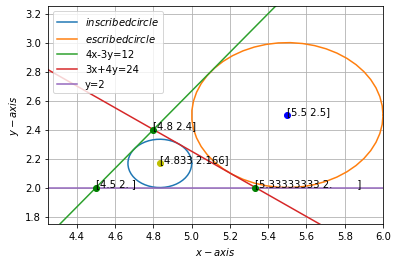
\includegraphics[width=\columnwidth]{assignment4/assignment4.png}
    \caption{This is the 2D diagram of the triangle , the inscribed circle and the escribed circle opposite to vertex $\vec{A}$}
    \label{myfig:1}
    \end{center}
\end{figure}
\end{document}
